


\section{\highlight[id=Yuge]{Circle and Rectangle}}


For simplicity, the centroid of shape in Fig.~\ref{fig:simple_imgs} is
located at the center of the image, although periodic boundary
conditions can eliminate the boundary and translation effects. Circle
and rectangle are simple convex shapes without sophisticated geometric
features. Moreover, it is well-known that the rectangle perimeter is
longer than the circle circumference when their areas are
identical. Therefore, in theory, survival probabilities at short
times, i.e. number of steps $n$, of particles in the image with a
rectangle are smaller than a circle.


    \begin{figure}
      \centering
      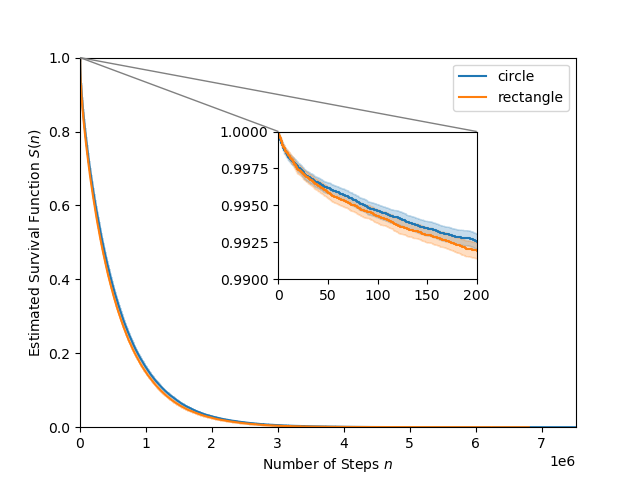
\includegraphics[width=\textwidth]{circle_rect_steps_sf.png}
      \caption{Since the survival curves for circle and rectangle overlap and cross, it is hard to detect the difference between them by eyes. However, the inset figure shows the greater details about the survival probabilities within the small number of steps. The area around the survival curve with the pale colour represents $95\%$ confidence interval.}
      \label{fig:sf_simple_shape_steps}
    \end{figure}


   \begin{figure}
      \centering
      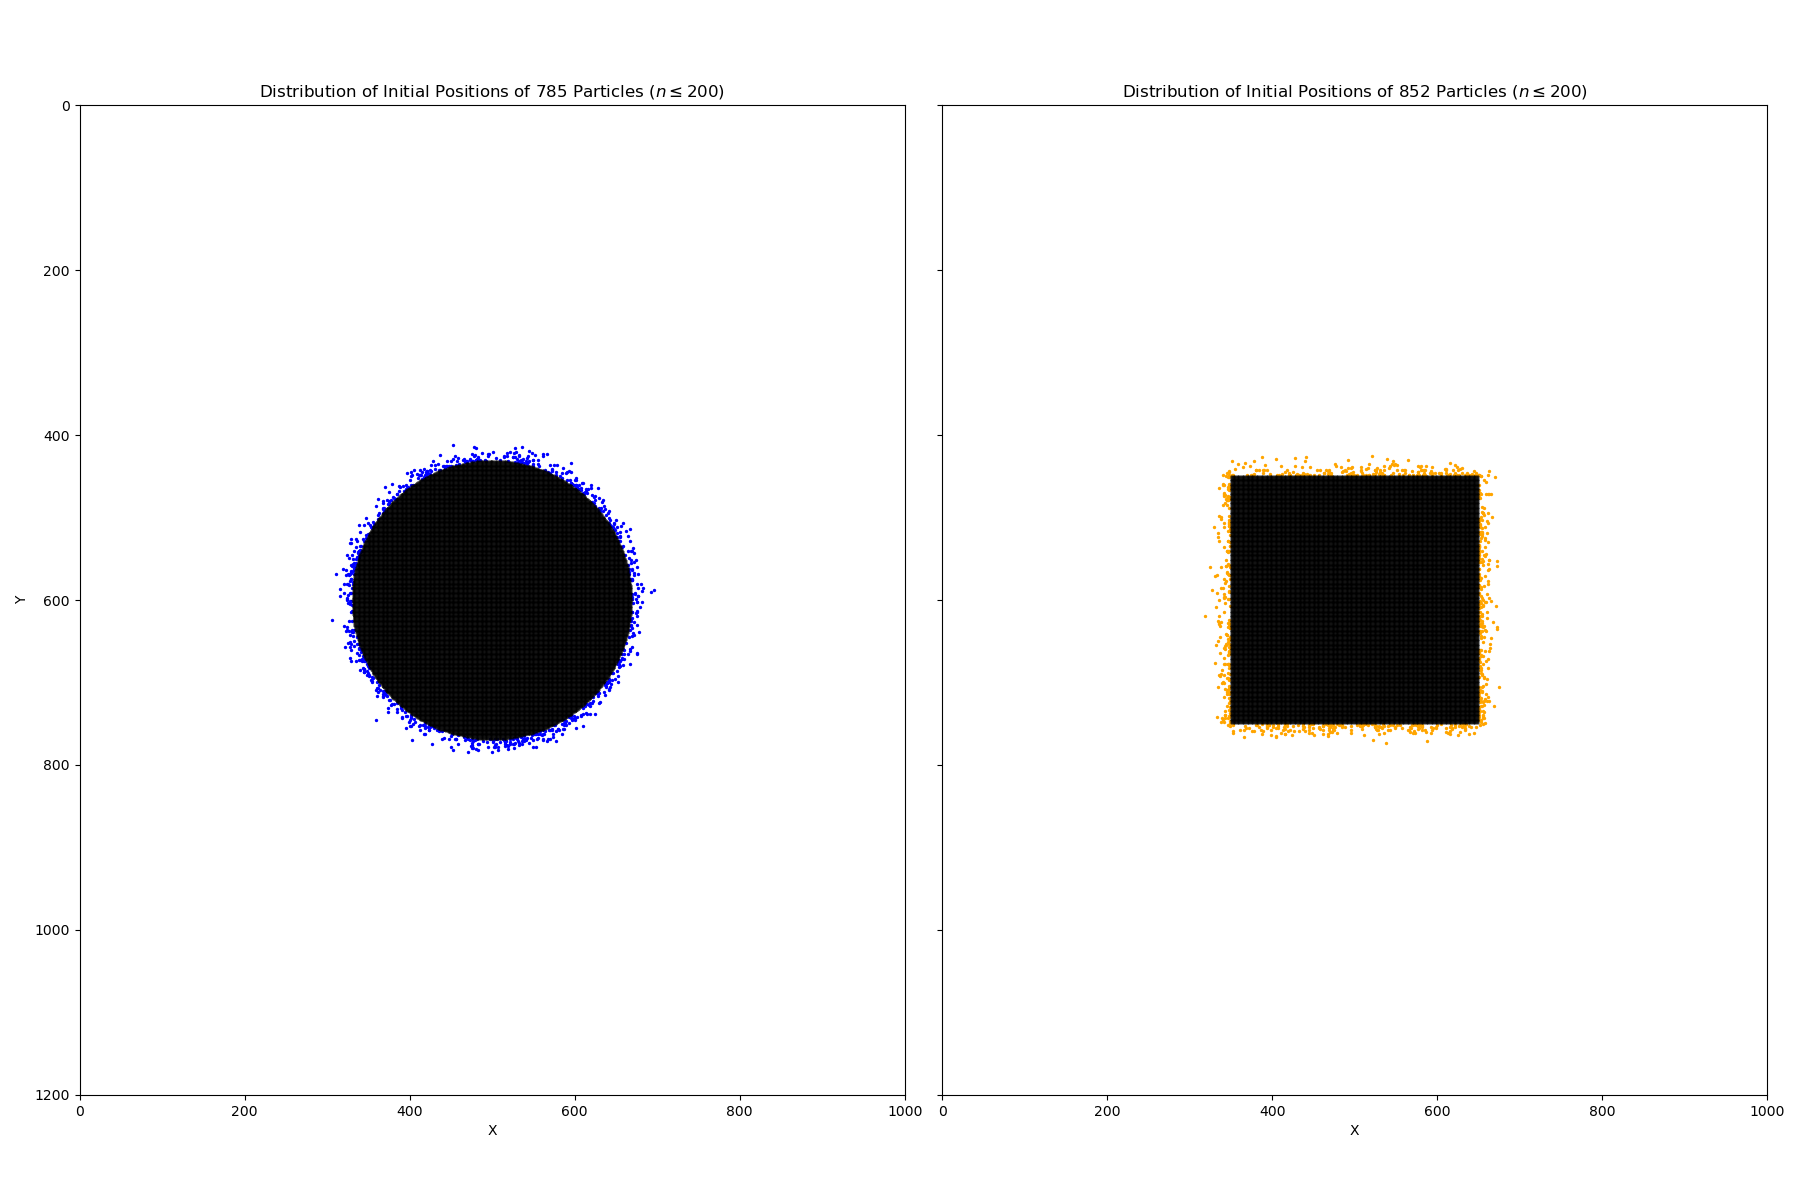
\includegraphics[width=\textwidth]{circle_rect_steps_initial_pos.png}
      \caption{The coloured points in the left and right subfigure represent the initial positions of particles in LRWs, whose number of steps less than or equal to $200$.}
      \label{fig:cir_rect_steps_initial_pos}
    \end{figure}


Fig.~\ref{fig:sf_simple_shape_steps} shows the Kaplan-Meier estimates
and the $95\%$ confidence intervals for the survival functions,
$S(n)$, of circle and rectangle. The approximated $95\%$ confidence
intervals of the survival functions overlay results from the sampling
errors. The survival function decays monotonically from $1$ to $0$. In
LRWs, particles' initial positions are distributed uniformly in the
unoccupied space in the image, so none of them can be absorbed by the
boundary of the target shape. Also, all the particles will finally
stop the random walk and can not survive because of the absorbing
boundary condition.


Overall, the differences between survival functions for the circle and
rectangle are not visible. Nevertheless, an inset in
Fig.~\ref{fig:sf_simple_shape_steps} helps visually identify distinct
short-term behaviours of survival functions for circle and rectangle,
which are consistent with the theoretical results. From the
concentrated spatial distribution of points illustrated in
Fig.~\ref{fig:cir_rect_steps_initial_pos}, we can find that if
particles start LRWs close to the target object in the image, they
will hit the absorbing boundary within a few steps. Alternatively, the
short-term survival function describes a region in the shape of an
approximate belt next to the target object. Furthermore, the point
cloud around the rectangle comprises more particles than the circle
resulting from the longer perimeter. 



After the short-term study, the entire survival curves of circle and
rectangle needed to be compared to validate LRWs further. As
introduced in section ~\ref{section:MC_heat_content}, some
conventional nonparametric tests in survival analysis assess the null
hypothesis that there is no difference in survival probabilities at
all number of steps $n$. Among those tests, the log-rank test results
are reliable if the assumption of proportional hazards is satisfied,
which can be inspected by looking at the graph
Fig.~\ref{fig:ph_test_simple_shapes} showing $\ln{(-\ln{S(n)})}$
against $\ln{(n)}$.


   \begin{figure}
     \centering
     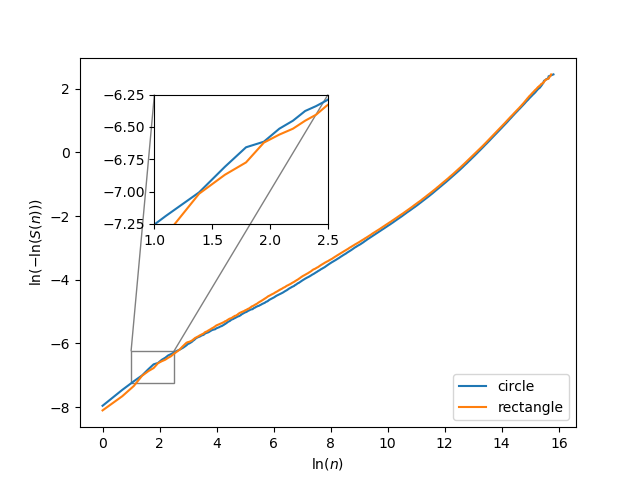
\includegraphics[width=\textwidth]{circle_rect_steps_ph.png}
     \caption{It is a graphical method for checking proportionality by looking for parallelism. The lines for circle and rectangle are not parallel since they cross at some points as shown in the inset, and the difference between them changes with logarithmically transformed $n$.}
     \label{fig:ph_test_simple_shapes}
   \end{figure}


  \begin{table}
     \centering
     \begin{tabular}{lrr}
        \toprule
         {} &  test\_statistic &             p \\
         \midrule
         log-rank & 137.23 & 0.0 \\
         \midrule
         Tarone-Ware & 134.31 & 0.0 \\
         \midrule
         Gehan-Breslow & 123.83 & 0.0 \\
         \midrule
         Fleming-Harrington & 123.83 & 0.0 \\
         \bottomrule
     \end{tabular}
     \caption{Survival functions for circle and rectangle are statistically different since p values equal zeros.}
     \label{tab:test_simple_shape_steps}
   \end{table}



The crossing lines with varying shapes in
Fig.~\ref{fig:ph_test_simple_shapes} suggest the rejection of the
proportional hazards assumption, and the log-rank test may loss
power. However, in Tab.~\ref{tab:test_simple_shape_steps}, log-rank,
Tarone-Ware, Gehan-Breslow, and Fleming-Harrington tests demonstrate
the rejection of the null hypothesis. In other words, there is a
statistically significant difference between the survival functions
for circle and rectangle. In conclusion, LRWs is an alternative
methodology to quantify and distinguish the regular simply connected
regions in the $2-$ dimensional image by developing and comparing the
corresponding survival functions.


  
